\chapter{Arhitektura i dizajn sustava}
		
		\textbf{\textit{dio 1. revizije}}\\



               \textit{Arhitektura sustava može se podijeliti  na tri podsustava: }

              \begin{packed_item}
               \item  Web  preglednik
                \item   Web aplikacija
                \item    Baza Podataka

                \end{packed_item}

                 \begin{figure}[H]
                     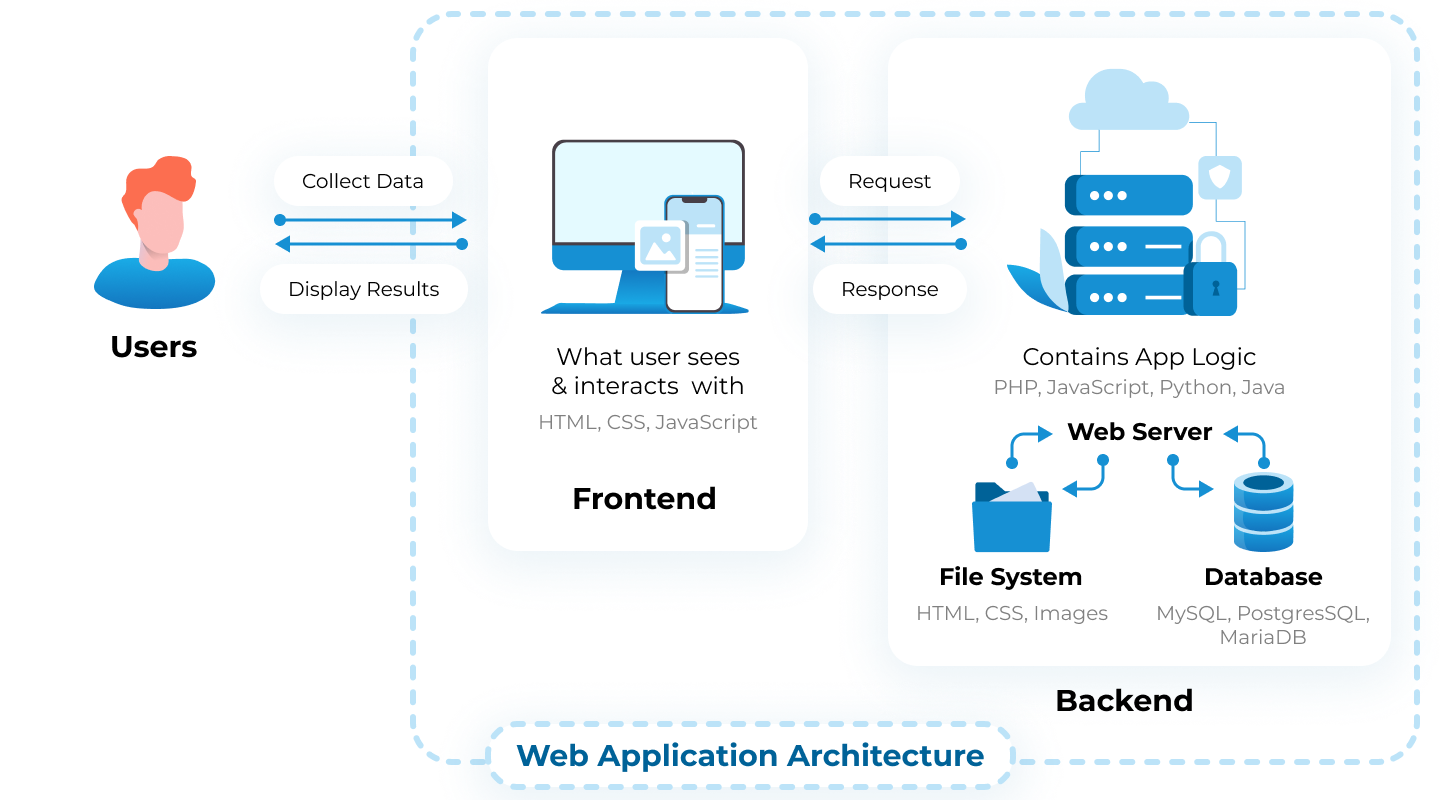
\includegraphics[width=7cm, height=5cm ]{./slike/arhitektura.png}
                      \centering
                      \caption{Arhitektura sustava}
                  \end{figure}


                  \textbf{Web preglednik} je aplikacija za prikaz web stranica. Kada korisnik posjeti neku web stranicu, internetski preglednik zatraži podatke
                                 sa web poslužitelja, koje interpretira i prikaže na zaslon računala ili nekog drugog pametnog uređaja.

                  \textbf{Web poslužitelj} osnovni podsustav u izradi web aplikacije. Njegova uloga u sustavu je komunikacija korisnika(web preglednika) s 
                                 aplikacijom. Komunikacija se ostvaruje preko HTTP (engl. Hyper Text Transfer Protocol) protokola. Uloga HTTP protokola je prijenos 
                                 sadržaja s poslužitelja na preglednik, koji dalje odrađuje svoj posao.
                            
                                Korisnik preko preglednika, koristi korisničko sučelje, te tako šalje HTTP zahtjeve na poslužitelj. Neki od zahtjeva su HTTP GET, HTTP POST 
                                itd. Svaki takav zahtjev u 99 \% slučajeva na poslužitelju izaziva, njegovu komunikaciju s \underbar{bazom podataka}.

                  \textbf{Baza podataka} je skup međusobno povezanih podataka, pohranjeni u vanjskoj memoriji računala. Njezina uloga u sustavu je brza i efikasna
                                 pohrana podataka, koji se propagiraju iz sloja web preglednika, preko web poslužitelja.

                  \textit{Web aplikacija se najčešće dijeli na dva dijela: }

                               \begin{packed_item}
              			 \item  \textbf{Front-end} koji je zadužen za razvoj korsicničkog iskustva na webu.
                		\item    \textbf{Back-end} koji je zadužen za obradu i spremanje podataka, koji dođu sa frontenda.

              		       \end{packed_item}

                                Tehnologije koje smo uzeli za razvoj web aplikacije su React.js za Front-end u razvojnom okruženju Microsoft Visual Studio Code, te .NET za Back-end u razvojnom okruženju Microsoft Visual Studio.
                                Uz .Net na back-endu, smo uzeli SQL server za bazu podataka. 
                                Arhitektura sustava će biti bazirana na MVC(engl. Model-View-Controller) konceptu.

                      \textbf{MVC} model sastoji se od tri komponenti: 
                                  
                               \begin{packed_item}
             			  \item \textbf{Model} -  komponenta modela koja je zadužena za dohvat i manipulacijom podataka. Često za obavljanje svojih zadaća koristi bazu podataka.
                		  \item  \textbf{View} -   komponenta kojoj je zadaća prikaz dobivenih podataka korisniku.
               		           \item  \textbf{Controller} - komponenta zadužena za primanje zahtjeva od korisnika, koje dalje propagira komponenti Model.

                                \end{packed_item}
                  
                    \begin{figure}[H]
                     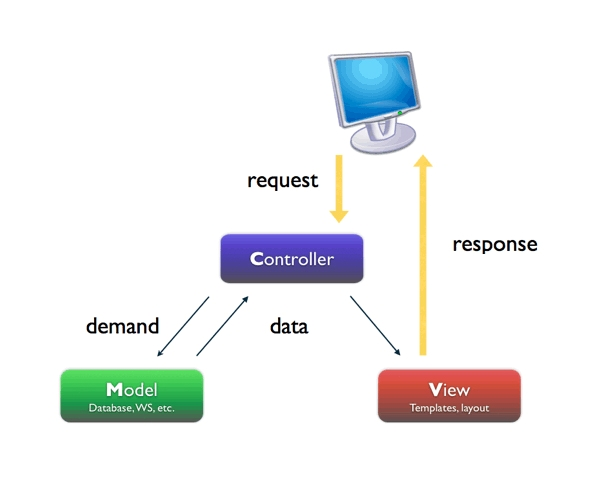
\includegraphics[width=7cm, height=5cm ]{./slike/mvc.jpg}
                      \centering
                      \caption{MVC model}
                    \end{figure}
                    
                                 

			
		\section{Baza podataka}
			
			\textbf{\textit{dio 1. revizije}}\\
			
		\textit{Potrebno je opisati koju vrstu i implementaciju baze podataka ste odabrali, glavne komponente od kojih se sastoji i slično.}
		
			\subsection{Opis tablica}
			

				\textit{Svaku tablicu je potrebno opisati po zadanom predlošku. Lijevo se nalazi točno ime varijable u bazi podataka, u sredini se nalazi tip podataka, a desno se nalazi opis varijable. Svjetlozelenom bojom označite primarni ključ. Svjetlo plavom označite strani ključ}
				

\textbf{Users} Ovaj entitet sadrži sve važne informacije o korisniku aplikacije. Sadrži atribute: korisničko ime, OIB, ime, prezime, fotografiju, broj telefona, adresu elektroničke pošte, lozinku, ID uloge korisnika te status je li potvrđen. Ovaj entitet u vezi je \textit{Many-to-One} s entitetom Role preko atributa identifikatora uloge, u vezi \textit{One-To-Many} s entitetom Operation preko atributa identifikatora osobe, u vezi \textit{One-to-Many} s entitetom Comment preko atributa identifikatora osobe, u vezi \textit{One-To-Many} s entitetom Area preko atributa identifikatora osobe te u vezi \textit{One-To-Many} s entitetom Block preko atributa identifikatora osobe. 
				\begin{longtblr}[
					label=none,
					entry=none
					]{
						width = \textwidth,
						colspec={|X[6,l]|X[6, l]|X[20, l]|}, 
						rowhead = 1,
					} %definicija širine tablice, širine stupaca, poravnanje i broja redaka naslova tablice
					\hline \multicolumn{3}{|c|}{\textbf{Users}}	 \\ \hline[3pt]
					Username & VARCHAR	&  	korisničko ime korisnika  	\\ \hline
					\SetCell{LightGreen}OIB	& BIGINT & jedinstveni identifikator osobe   	\\ \hline 
					FirstName & VARCHAR & ime korisnika  \\ \hline 
					LastName & VARCHAR	& prezime korisnika 		\\ \hline
					Photo & VARCHAR & fotografija korisnika \\ \hline 
				    PhoneNumber & VARCHAR & telefonski broj korisnika  	\\ \hline 
					EMail & VARCHAR & adresa elektroničke pošte korisnika  	\\ \hline
					Password & VARCHAR & hash lozinke  	\\ \hline
                    \SetCell{LightBlue}RoleId & INT & identifikator uloge  	\\ \hline
                    Confirmed & BIT & status je li administrator potvrdio korisnika  	\\ \hline
				\end{longtblr}
				
\textbf{Role} Ovaj entitet sadrži sve važne informacije o ulogama korisnika aplikacije. Sadrži atribute ID uloge i ime uloge. Ovaj entitet u vezi je \textit{One-to-Many} s entitetom Users preko atributa identifikatora uloge. 
				\begin{longtblr}[
					label=none,
					entry=none
					]{
						width = \textwidth,
						colspec={|X[6,l]|X[6, l]|X[20, l]|}, 
						rowhead = 1,
					} %definicija širine tablice, širine stupaca, poravnanje i broja redaka naslova tablice
					\hline \multicolumn{3}{|c|}{\textbf{Role}}	 \\ \hline[3pt]
					\SetCell{LightGreen}Id & INT	&  jedinstveni identifikator uloge  	\\ \hline
					Name	& VARCHAR &  naziv uloge 	\\ \hline
				\end{longtblr}
			
\textbf{Missing Report} Ovaj entitet sadrži sve važne informacije o prijavama nestalih osoba. Sadrži atribute: ID prijave, ime osobe, prezime osobe, OIB osobe, fotografiju osobe, opis prijave, datum i vrijeme prijave te datum i vrijeme pronalaska. Ovaj entitet u vezi je \textit{One-to-Many} s entitetom Comment preko atributa identifikatora prijave nestale osobe.  
				\begin{longtblr}[
					label=none,
					entry=none
					]{
						width = \textwidth,
						colspec={|X[6,l]|X[6, l]|X[20, l]|}, 
						rowhead = 1,
					} %definicija širine tablice, širine stupaca, poravnanje i broja redaka naslova tablice
					\hline \multicolumn{3}{|c|}{\textbf{Missing Report}}	 \\ \hline[3pt]
					\SetCell{LightGreen}Id & INT	&  jedinstveni identifikator prijave nestale osobe  	\\ \hline
					FirstName	& VARCHAR &  ime nestale osobe 	\\ \hline
                    LastName	& VARCHAR &  prezime nestale osobe 	\\ \hline
                    OIB	& BIGINT &  jedinstveni identifikator nestale osobe 	\\ \hline
                    Photo	& VARCHAR &  fotografija nestale osobe 	\\ \hline
                    Description	& VARCHAR &  opis prijave nestale osobe 	\\ \hline
                    ReportedAt & DATETIME & datum i vrijeme prijave nestanka osobe   \\ \hline
                    FoundAt & DATETIME & datum i vrijeme pronalaska nestale osobe \\ \hline
				\end{longtblr}
			
\textbf{Comment} Ovaj entitet sadrži sve važne informacije o komentarima prijava nestalih osoba. Sadrži atribute ID komentara, ID prijave koja se komentira, sadržaj komentara, OIB korisnika. Ovaj entitet u vezi je \textit{Many-to-One} s entitetom Missing Report preko atributa identifikatora prijave nestale osobe i u vezi \textit{Many-to-One} s entitetom Users preko atributa identifikatora osobe. 
				\begin{longtblr}[
					label=none,
					entry=none
					]{
						width = \textwidth,
						colspec={|X[6,l]|X[6, l]|X[20, l]|}, 
						rowhead = 1,
					} %definicija širine tablice, širine stupaca, poravnanje i broja redaka naslova tablice
					\hline \multicolumn{3}{|c|}{\textbf{Comment}}	 \\ \hline[3pt]
					\SetCell{LightGreen}Id & INT	&  jedinstveni identifikator komentara  	\\ \hline
					\SetCell{LightBlue}ReportId	& INT &  jedinstveni identifikator prijave nestale osobe 	\\ \hline
                    Text & VARCHAR &  sadržaj komentara 	\\ \hline
                    \SetCell{LightBlue} UserOIB	& BIGINT &  jedinstveni identifikator osobe koja komentira 	\\ \hline
				\end{longtblr}

\textbf{Operation} Ovaj entitet sadrži sve važne informacije o operacijama. Sadrži atribute: ID operacije, status operacije i OIB voditelja operacije. Ovaj entitet u vezi je \textit{Many-to-One} s entitetom Users preko atributa identifikatora osobe te u vezi \textit{One-To-Many} s entitetom Region preko atributa identifikatora operacije. 
				\begin{longtblr}[
					label=none,
					entry=none
					]{
						width = \textwidth,
						colspec={|X[6,l]|X[6, l]|X[20, l]|}, 
						rowhead = 1,
					} %definicija širine tablice, širine stupaca, poravnanje i broja redaka naslova tablice
					\hline \multicolumn{3}{|c|}{\textbf{Operation}}	 \\ \hline[3pt]
					\SetCell{LightGreen}Id & INT	&  jedinstveni identifikator operacije\\ \hline
					Status	& VARCHAR &  status operacije 	\\ \hline
                    \SetCell{LightBlue}LeaderOIB	& BIGINT & jedinstveni identifikator voditelja operacije 	\\ \hline
				\end{longtblr}


\textbf{Area} Ovaj entitet sadrži sve važne informacije o područjima. Sadrži atribute: identifikator područja, datum i vrijeme nastanka područja, datum i vrijeme zatvaranja područja te identifikator osobe koja je zadnja uređivala područje. Ovaj entitet u vezi je \textit{Many-to-One} s entitetom Users preko atributa identifikatora osobe, u vezi \textit{One-To-Many} s entitetom Block preko atributa identifikatora područja, u vezi \textit{One-To-Many} s entitetom Building preko atributa identifikatora područja, u vezi \textit{One-To-Many} s entitetom Point preko atributa identifikatora područja te u vezi \textit{One-To-Many} s entitetom Region preko atributa identifikatora područja. 
				\begin{longtblr}[
					label=none,
					entry=none
					]{
						width = \textwidth,
						colspec={|X[9,l]|X[6, l]|X[20, l]|}, 
						rowhead = 1,
					} %definicija širine tablice, širine stupaca, poravnanje i broja redaka naslova tablice
					\hline \multicolumn{3}{|c|}{\textbf{Area}}	 \\ \hline[3pt]
					\SetCell{LightGreen}Id & INT	&  jedinstveni identifikator područja \\ \hline
					CreatedAt & DATETIME & datum i vrijeme nastanka područja \\ \hline
					ClosedAt & DATETIME & datum i vrijeme zatvaranja područja \\ \hline
					\SetCell{LightBlue}UpdatedLastByOIB	& BIGINT &  identifikator osobe koja je zadnja uređivala područje 	\\ \hline
				\end{longtblr}  
                
\textbf{Region} Ovaj entitet sadrži sve važne informacije o regiji. Sadrži atribute: identifikator regije te identifikator operacije. Ovaj entitet u vezi je \textit{Many-to-One} s entitetom Area preko atributa identifikatora regije, u vezi \textit{Many-To-One} s entitetom Operation preko atributa identifikatora operacije te u vezi \textit{One-To-Many} s entitetom Block preko atributa identifikatora regije. 
				\begin{longtblr}[
					label=none,
					entry=none
					]{
						width = \textwidth,
						colspec={|X[6,l]|X[6, l]|X[20, l]|}, 
						rowhead = 1,
					} %definicija širine tablice, širine stupaca, poravnanje i broja redaka naslova tablice
					\hline \multicolumn{3}{|c|}{\textbf{Region}}	 \\ \hline[3pt]
					\SetCell{LightGreen}AreaId & INT	&  jedinstveni identifikator regije \\ \hline
					\SetCell{LightBlue}OperationId	& INT &  jedinstveni identifikator operacije 	\\ \hline
				\end{longtblr}            
				
\textbf{Block} Ovaj entitet sadrži sve važne informacije o blokovima. Sadrži atribute: identifikator bloka, status bloka, identifikator regije te identifikator osobe koja uređuje blok. Ovaj entitet u vezi je \textit{Many-to-One} s entitetom Users preko atributa identifikatora osobe, u vezi \textit{Many-To-One} s entitetom Area preko atributa identifikatora bloka, u vezi \textit{Many-To-One} s entitetom Region preko atributa identifikatora regije te u vezi \textit{One-To-Many} s entitetom Building preko atributa identifikatora bloka. 
	          \begin{longtblr}[
	          	label=none,
	          	entry=none
	          	]{
	          		width = \textwidth,
	          		colspec={|X[6,l]|X[6, l]|X[20, l]|}, 
	          		rowhead = 1,
	          	} %definicija širine tablice, širine stupaca, poravnanje i broja redaka naslova tablice
	          	\hline \multicolumn{3}{|c|}{\textbf{Block}}	 \\ \hline[3pt]
	          	\SetCell{LightGreen}AreaId & INT	&  jedinstveni identifikator bloka \\ \hline
	          	Status & VARCHAR & status bloka \\ \hline
	          	\SetCell{LightBlue}RegionId & INT & jedinstveni identifikator regije \\ \hline
	          	\SetCell{LightBlue}ActiveForOIB	& BIGINT &  identifikator kartografa koji trenutno uređuje blok 	\\ \hline
	          \end{longtblr}  
				
\textbf{Building} Ovaj entitet sadrži sve važne informacije o građevinama. Sadrži atribute: identifikator građevine, identifikator bloka te status građevine. Ovaj entitet u vezi je \textit{Many-to-One} s entitetom Area preko atributa identifikatora građevine te u vezi \textit{Many-To-One} s entitetom Block preko atributa identifikatora bloka.
			\begin{longtblr}[
				label=none,
				entry=none
				]{
					width = \textwidth,
					colspec={|X[6,l]|X[6, l]|X[20, l]|}, 
					rowhead = 1,
				} %definicija širine tablice, širine stupaca, poravnanje i broja redaka naslova tablice
				\hline \multicolumn{3}{|c|}{\textbf{Building}}	 \\ \hline[3pt]
				\SetCell{LightGreen}AreaId & INT	&  jedinstveni identifikator građevine \\ \hline
				\SetCell{LightBlue}BlockId & INT & jedinstveni identifikator bloka \\ \hline
	          	Status & VARCHAR & status građevine \\ \hline
			\end{longtblr}

\textbf{Point} Ovaj entitet sadrži sve važne informacije o točkama i njihovim koordinatama. Sadrži atribute: identifikator točke, geografska širina, geografska dužina, identifikator područja te redni broj. Ovaj entitet u vezi je \textit{Many-to-One} s entitetom Area preko atributa identifikatora područja.
			\begin{longtblr}[
				label=none,
				entry=none
				]{
					width = \textwidth,
					colspec={|X[6,l]|X[6, l]|X[20, l]|}, 
					rowhead = 1,
				} %definicija širine tablice, širine stupaca, poravnanje i broja redaka naslova tablice
				\hline \multicolumn{3}{|c|}{\textbf{Point}}	 \\ \hline[3pt]
				\SetCell{LightGreen}Id & INT	&  jedinstveni identifikator točke \\ \hline
				Latitude & FLOAT & geografska širina točke \\ \hline
				Longitude & FLOAT & geografska dužina točke \\ \hline
				\SetCell{LightBlue}AreaId & INT & jedinstveni identifikator područja \\ \hline
				OrderNumber & INT & redni broj točke \\ \hline
			\end{longtblr}
			
			\subsection{Dijagram baze podataka}
				\begin{figure}[H]
					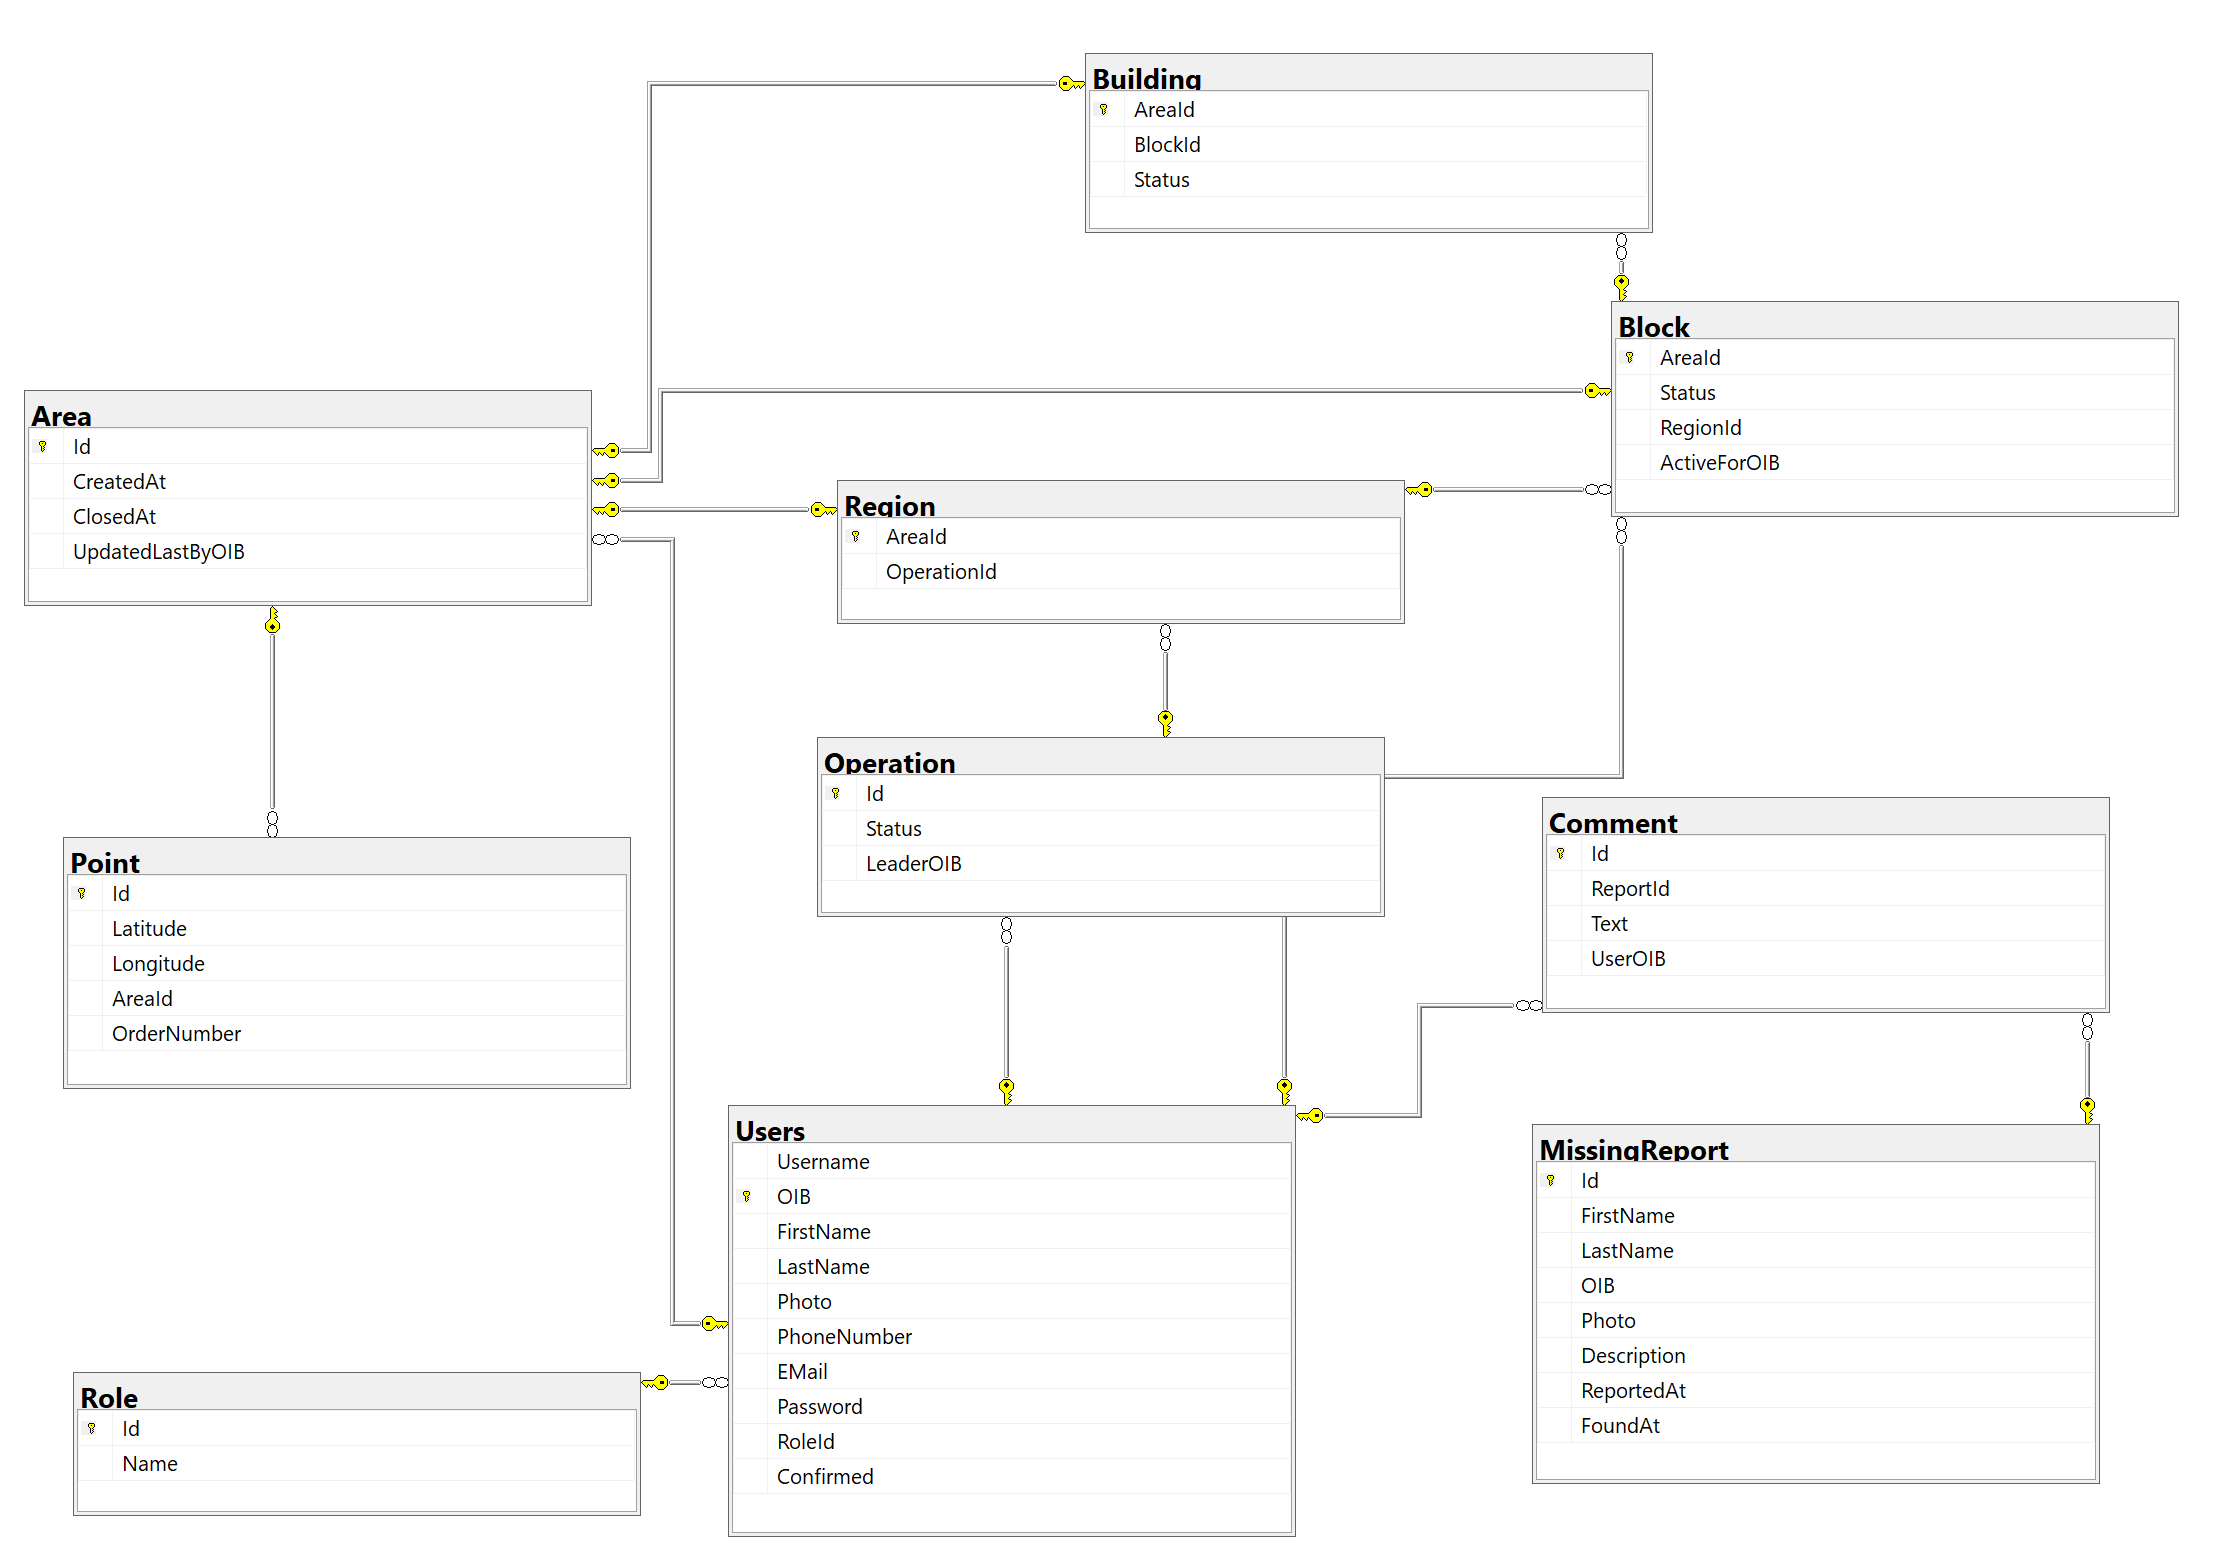
\includegraphics[width=15cm]{./slike/ERDijagram.png}
					 \centering
					 \caption{ER dijagram baze podataka}
				\end{figure}
			\eject
			
			
		\section{Dijagram razreda}
		
			\textit{Potrebno je priložiti dijagram razreda s pripadajućim opisom. Zbog preglednosti je moguće dijagram razlomiti na više njih, ali moraju biti grupirani prema sličnim razinama apstrakcije i srodnim funkcionalnostima.}\\
			
			\textbf{\textit{dio 1. revizije}}\\
			
			\begin{figure}[h!] 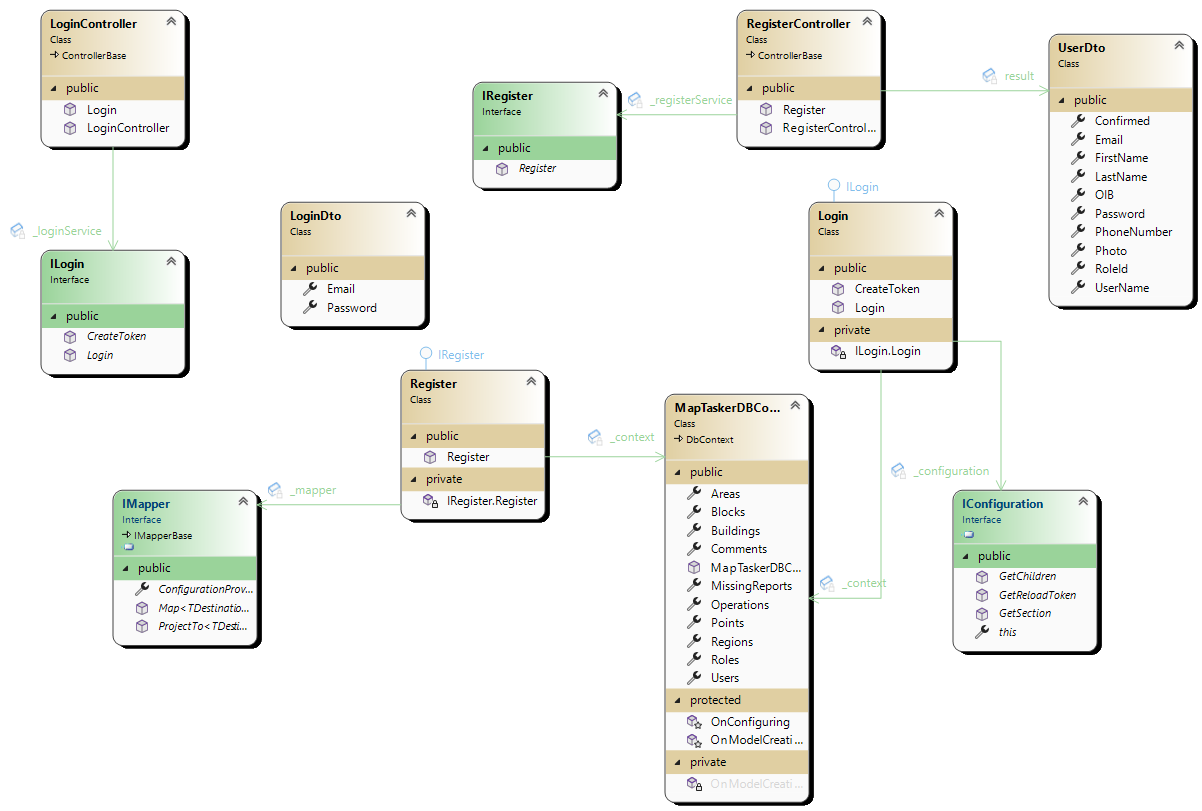
\includegraphics[width=\linewidth]{dijagrami/CD-LoginRegister.png}
				\caption{Dijagram razreda 1 - Register i Login}
			\end{figure}
		
			\begin{figure}[h!] 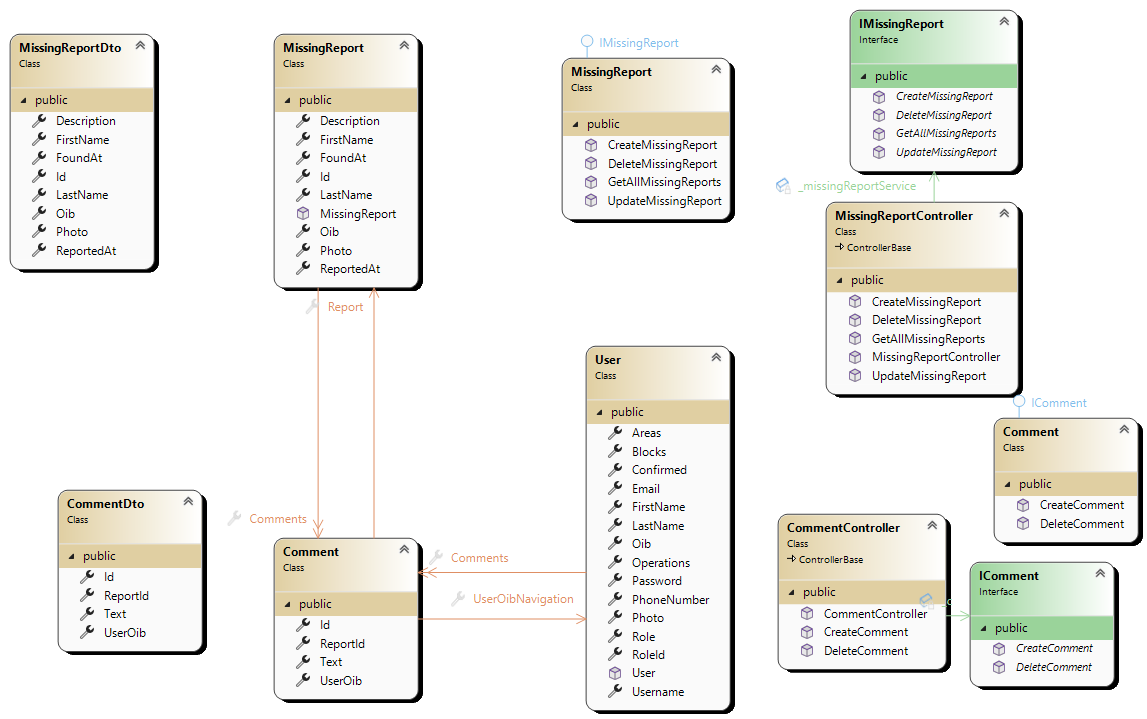
\includegraphics[width=\linewidth]{dijagrami/CD-CommentMissingReport.png}
				\caption{Dijagram razreda 2 - Missing Report i Comment}
			\end{figure}
		
			\begin{figure}[h!] 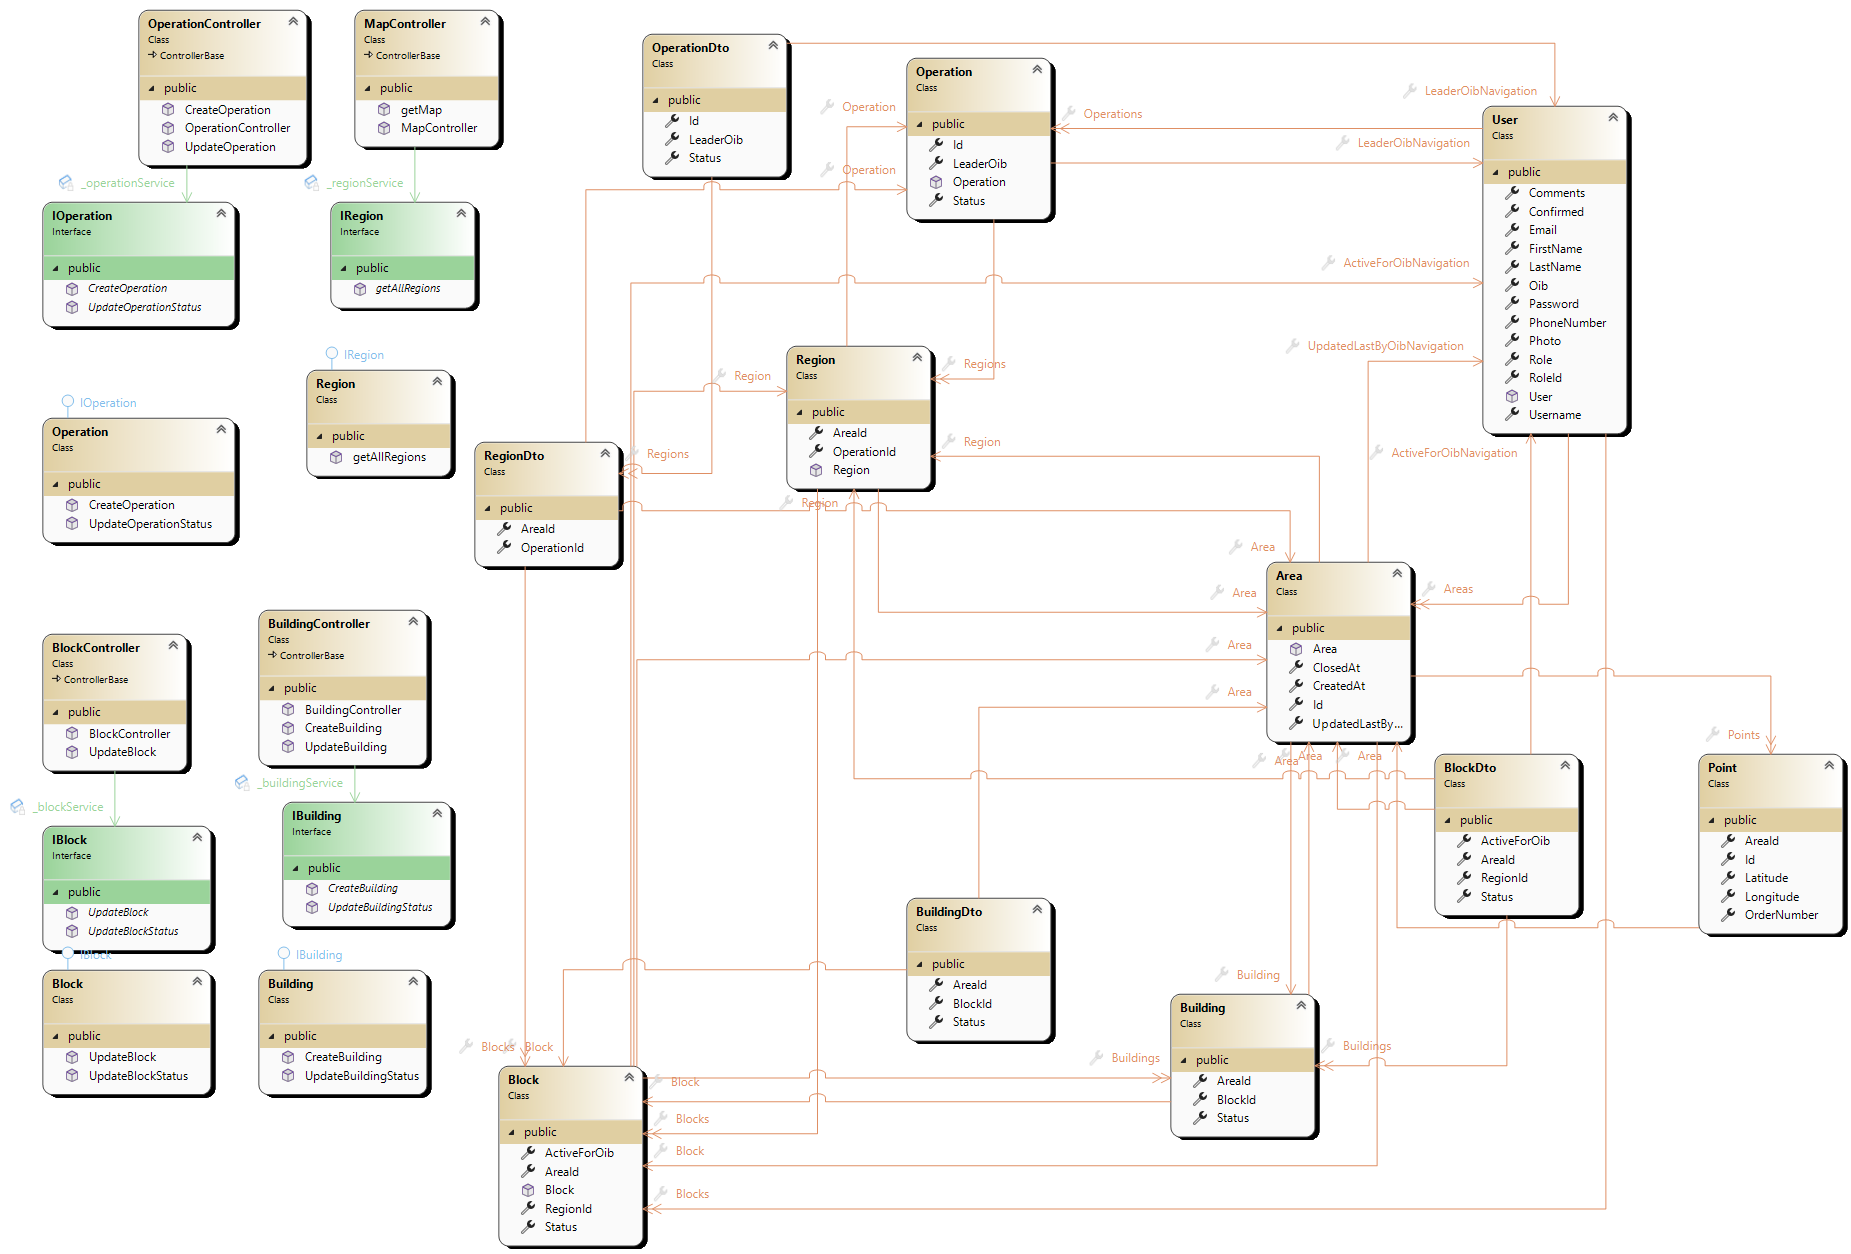
\includegraphics[width=\linewidth]{dijagrami/CD-AreasOperations.png}
				\caption{Dijagram razreda 3 - Operations, Areas, Regions, Blocks, Buildings}
			\end{figure}
		
			\begin{figure}[h!] 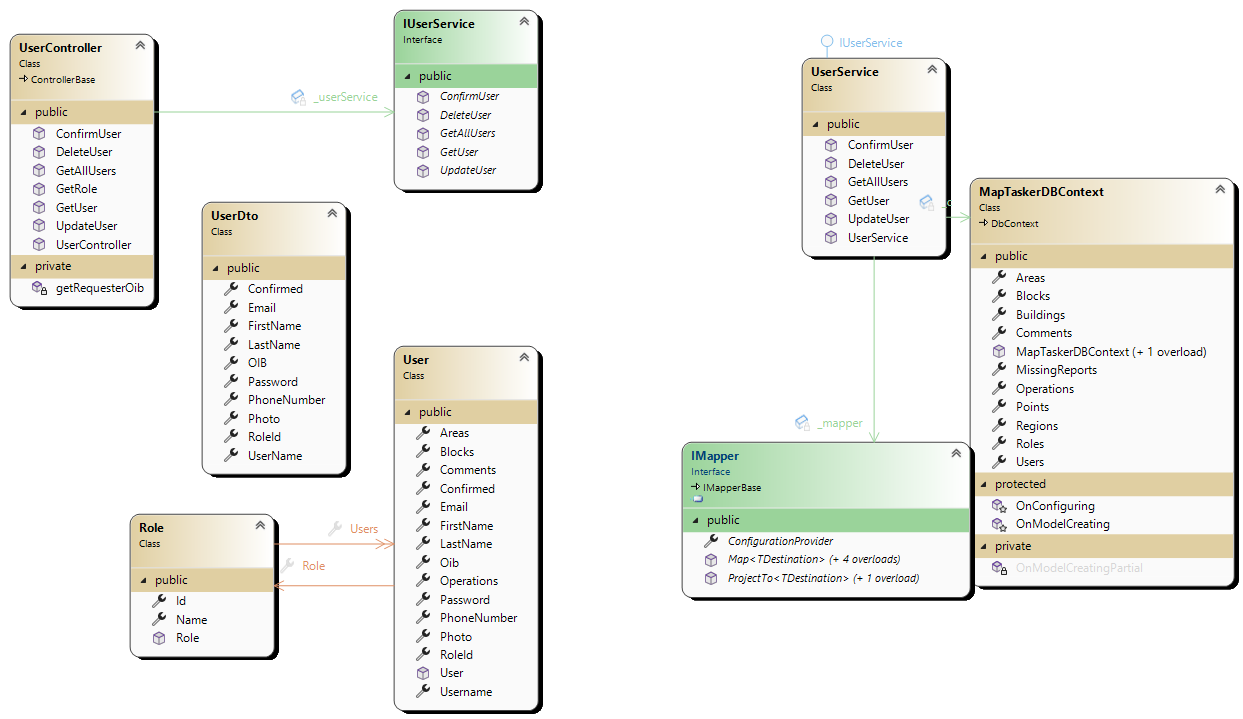
\includegraphics[width=\linewidth]{dijagrami/CD-UserRole.png}
				\caption{Dijagram razreda 4 - User i Role}
			\end{figure}
		
			\begin{figure}[h!] 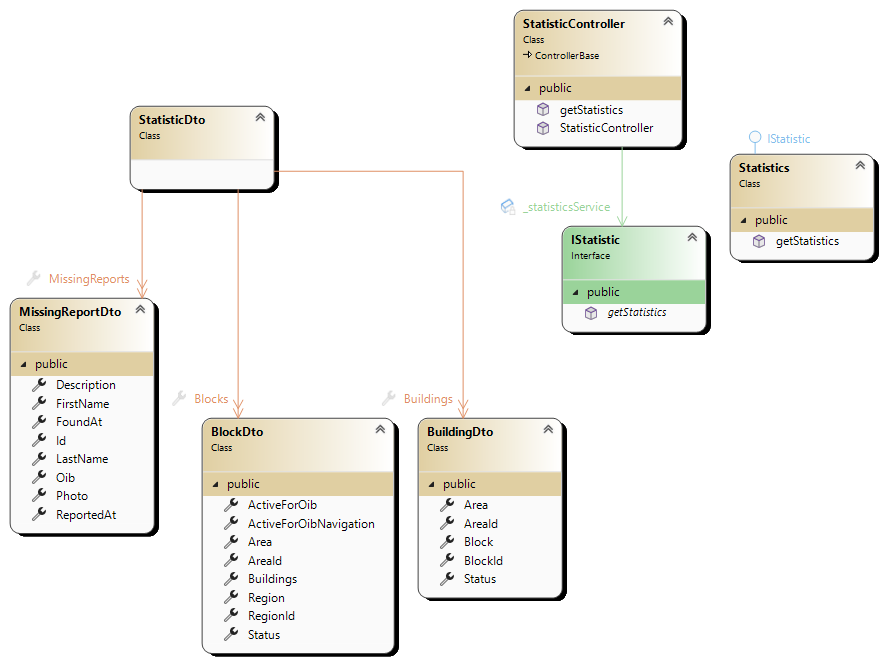
\includegraphics[width=\linewidth]{dijagrami/CD-Statistics.png}
				\caption{Dijagram razreda 5 - Statistics}
			\end{figure}
			
			\textit{Prilikom prve predaje projekta, potrebno je priložiti potpuno razrađen dijagram razreda vezan uz \textbf{generičku funkcionalnost} sustava. Ostale funkcionalnosti trebaju biti idejno razrađene u dijagramu sa sljedećim komponentama: nazivi razreda, nazivi metoda i vrste pristupa metodama (npr. javni, zaštićeni), nazivi atributa razreda, veze i odnosi između razreda.}\\
			
			\textbf{\textit{dio 2. revizije}}\\			
			
			\textit{Prilikom druge predaje projekta dijagram razreda i opisi moraju odgovarati stvarnom stanju implementacije}
			
			
			
			\eject
		
		\section{Dijagram stanja}
			
			
			\textbf{\textit{dio 2. revizije}}\\
			
			\textit{Potrebno je priložiti dijagram stanja i opisati ga. Dovoljan je jedan dijagram stanja koji prikazuje \textbf{značajan dio funkcionalnosti} sustava. Na primjer, stanja korisničkog sučelja i tijek korištenja neke ključne funkcionalnosti jesu značajan dio sustava, a registracija i prijava nisu. }
			
			
			\eject 
		
		\section{Dijagram aktivnosti}
			
			\textbf{\textit{dio 2. revizije}}\\
			
			 \textit{Potrebno je priložiti dijagram aktivnosti s pripadajućim opisom. Dijagram aktivnosti treba prikazivati značajan dio sustava.}
			
			\eject
		\section{Dijagram komponenti}
		
			\textbf{\textit{dio 2. revizije}}\\
		
			 \textit{Potrebno je priložiti dijagram komponenti s pripadajućim opisom. Dijagram komponenti treba prikazivati strukturu cijele aplikacije.}
